\section{Introduction}

The authors of the seminal Sugarscape model \cite{epstein_growing_1996} explicitly advocate object-oriented programming as "a particularly natural development environment for Sugarscape specifically and artificial societies generally.". They implemented their simulation software in Object Pascal and C where they used the former for programming the agents and the latter for low-level graphics \cite{axtell_aligning_1996}. Axelrod \cite{axelrod_advancing_1997} recommends Java for experienced programmers and Visual Basic for beginners. Up until now most of the ABS community seems to have followed these suggestions and are implemented using programming languages of the object-oriented imperative paradigm.

In this paper we challenge these suggestions and ask how agent-based simulation can be implemented in the pure functional programming language Haskell. 

A serious problem of object-oriented implementations is the blurring of the fundamental difference between agent and object - an agent is first of all a metaphor and \textit{not} an object. In object-oriented programming this distinction is obviously lost as in such languages agents are implemented as objects which leads to the inherent problem that one automatically reasons about agents in a way as they were objects - agents have indeed become objects in this case. The most notable difference between an agent and an object is that the latter one do not encapsulate behaviour activation \cite{jennings_agent-based_2000} - it is passive. Also it is remarkable that \cite{jennings_agent-based_2000} a paper from 1999 claims that object-orientation is not well suited for modelling complex systems because objects behaviour is too fine granular and method invocation a too primitive mechanism.

In \cite{axelrod_chapter_2006} Axelrod reports the vulnerability of ABS to misunderstanding. Due to informal specifications of models and change-requests among members of a research-team bugs are very likely to be introduced. He also reported how difficult it was to reproduce the work of \cite{axelrod_convergence_1995} which took the team four months which was due to inconsistencies between the original code and the published paper. The consequence is that counter-intuitive simulation results can lead to weeks of checking whether the code matches the model and is bug-free as reported in \cite{axelrod_advancing_1997}. As ABS is almost always used for scientific research, producing often break-through scientific results as pointed out in \cite{axelrod_chapter_2006} and used for policy making, these ABS need to be \textit{free of bugs}, \textit{verified against their specification}, \textit{validated against hypotheses} and ultimately be \textit{reproducible}.

Pure functional programming in Haskell claims \cite{hudak_history_2007}, \cite{hudak_haskell_1994} to overcome these problems or at least allows to tackle them more effectively due to its declarative nature, free of side-effects, strong static type system. 

TODO: aim 
TODO: objective
TODO: outcome 
TODO: contribution

\subsection{Costy bugs due to language features}
[ ] knight capital glitch
[ ] mars lander
[ ] moon landing
[ ] ?
[ ] ethereum \& blockchain technology

- The 3 major benefits of the approach I claim
	1. code == spec
	2. can rule out serious class of bugs
	3. we can perform reasoning about the simulation in code
	need to be metricated: e.g. this is really only possible in Haskell and not in Java. This needs thorough thinking about which metrics are used, how they can be aquired, how they can be compared,...
	
- I NEED TO SHOW HOW I CAN MAKE HASKELL RELEVANT IN THE FIELD OF ABS
	-> as far as I know so far no reasoning has been done in the way I intend to do it in the field of ABS. My hypothesis is that it is really only possible in Haskell due to its explicit side-effects, type-system, declarative style,... 
		-> TODO: need to check if this is really unique to haskell
	-> the functional-reactive approach seems to bring a new view to ABS with an embedded language for explicit time-semantics. Together with parallel/sequential updating this allows implementing System-Dynamics and agents which rely on continuous time-semantics e.g. SIR-Agents. Maybe i invented a hybrid between SD and ABS? Also what about time-traveling? The problem is that this is not really clear as i hypothesize that is completely novel approach to ABS - again I need to check this!
		-> TODO: is this really unique to functional reactive? E.g. what about Repast, NetLogo, AnyLogic, other Java-Frameworks? 
	-> maybe i have to admit that its not as unique as thought\\
	
In General i need to show that
- Haskells general benefits \& drawbacks over other Languages in the Field of ABS (e.g. Java, NetLogo, Repast) e.g. declarative style, reasoning, explicit about side-effects, performance, difficult to reason about performance, space-leaks difficult. So this focuses on the general comparison between the established technologies of ABS and Haskell but not yet on Haskells suitability in comparison to these other technologies. Here we talk about reasoning, side-effects, performance IN GENERAL TERMS, NOT SPECIFIC TO ABS. We need to distinguish between 
	-> general technicalities e.g. lambda-calculus (denotational formalism) or turing-machine (operational formalism) foundations, declarative style, lazy-evaluation allows to split the producer from the consumer, explicit about side-effects, not possible for in-order updates,...
	-> and in what they result e.g. fewer lines of code, ruling out of bugs, reasoning, lower performance, difficult to reason about space-time 
	
- Haskells suitability to implement ABS in comparison to other languages and technologies in the Field. Here the focus is on general problems in ABS and how they can and are solved using Haskell e.g. send message, changing environment, handling of time, replications, parallelism/concurrency,...

- Why using Haskell in ABS - do the general benefits / drawbacks apply equally well? Are there unique advantages? Can we do things in Haskell which are not possible in other technologies or just very hard? E.g. the hybrid-approach I created with FRP: how unique is it e.g. can other technologies easily implement it as well? Other potential advantages: recursive simulation. Here we DO NOT concentrate on general technicalities but see how they apply when using it for ABS and if they create a unique benefit for Haskell in ABS.

i need to show that different programming languages and paradigms have different power and are differently well suited to specific problems: the ultimate claim i need to show is that haskell is more powerful than java or C++ - the question is if this also makes it superior in applying it to problems: being more powerful, can all problems of java be solved better in haskell as well? this is i believe not the case e.g. gui- or game- programming. the question then is: what is the power of a programming language? can we measure it?

so what i need to show is how well haskell and its power are suited for implementing ABS. does the fact that haskell is much more powerful than existing technologies in ABS lead to the point that it is better suited for ABS? in fact it is power vs. better suited

\subsection{The power of a language}
[ ] more expressive: we can express complex problems more directly and with less  overhead. note that this is domain-specifix: the mechanisms of a language allow to create abstractions which solve the domain-specific problem. the better these mechanisms support one in this task, the more powerful the language is in the given domain. now we end up by defining what "better" support means
[ ] one could in pronciple do system programming in haskell by provoding bindings to code written in c and / or assembly but when the program is dominated by calls to these bindings then one could as well work directly in these lower languages and saves one from the overhead of the bindings
[ ] but very often a domain consists of multiple subdomains.
[ ] my hypothesis is that haskell is not well suited for domains which are dominated by managing and manipulating a global mutable state through side-effects / effectful computations. examples are gui-programming and computer games (state spread accross GPU and cpu, user input,...). this does not mean that it is not possible to implememt these things in haskell (it has been done with some sucess) but that the solution becomes too complex at some point.
[ ] conciesness
[ ] low ceremony
[ ] susceptibility to bugs
[ ] verbosity
[ ] reasoning about performance
[ ] reasoning about space requirements

\subsection{Measuring a language}
Define scientific measures: e.g. Lines Of Code (show relation to Bugs \& Defects, which is an objective measure: http://www.stevemcconnell.com/est.htm, \url{https://softwareengineering.stackexchange.com/questions/185660/is-the-average-number-of-bugs-per-loc-the-same-for-different-programming-languag}, Book: Code Complete, \url{https://www.mayerdan.com/ruby/2012/11/11/bugs-per-line-of-code-ratio}), also experience reports by companies which show that Haskell has huge benefits when applied to the same domain of a previous implementation of a different language, post on stack overflow / research gate / reddit, read experience reports from \url{http://cufp.org/2015/} Also need to show the problem of operational reasoning as opposed to denotational reasoning

\subsection{The Abstraction Hierarchy}

1st: Functional vs. Object Oriented
2nd: Haskell vs. Java
3rd: FrABS vs. Repast

\subsection{Drawbacks}
the way the statechart is implemente in RePast requires that agents expose data through public methods or variables which exposes much more information than really needed.

\section{Background}

\subsection{Agent-Based Simulation}
We understand ABS as a method of modelling and simulating a system where the global behaviour may be unknown but the behaviour and interactions of the parts making up the system is of knowledge. Those parts, called agents, are modelled and simulated out of which then the aggregate global behaviour of the whole system emerges. So the central aspect of ABS is the concept of an agent which can be understood as a metaphor for a pro-active unit, situated in an environment, able to spawn new agents and interacting with other agents in a network of neighbours by exchange of messages \cite{wooldridge_introduction_2009}. It is important to note that we focus our understanding of ABS on a very specific kind of agents where the focus is on communicating entities with individual, localized behaviour from out of which the global behaviour of the system emerges. We informally assume the following about our agents:

\begin{itemize}
	\item They are uniquely addressable entities with some internal state over which they have full, exclusive control.
	\item They are pro-active which means they can initiate actions on their own e.g. change their internal state, send messages, create new agents, terminate themselves.
	\item They are situated in an environment and can interact with it.
	\item They can interact with other agents which are situated in the same environment by means of message-passing.
\end{itemize} 

\subsection{Implementation}
The challenges one faces when implementing an ABS plain, without support from a library are manifold. Generally one faces the following challenges:

\begin{itemize}
	\item Agent Representation - how do we represent an agent? The ABS community implements agents as objects (as in Java, Python or C++) as they claim that the mapping of an agent on an object is natural. The question is how to represent an agent in Haskell?
	\item Agent-Agent Interaction - how can agents interact with other agents? In object-orientation we have method-calls which allows to call other objects and mutate their state. Also this is not available in Haskell, so how do we solve this problem without resorting to the IO monad?
	\item Environment representation - how can we represent an environment? Also an environment must have the ability to update itself e.g. regrow some resources.
	\item Agent-Environment interaction - how can agents interact (read / write) with the environment they are situated in?
	\item Agent Updating - how is the set of agents organised, how are they updated and how is it managed (deleting, adding during simulation)? In object-oriented implementations due to side-effects and mutable data in-order updates are easily done but this is not available in Haskell without resorting to the IO monad.
\end{itemize}

\subsection{SIR Model}
- do not introduce SIR model in that length, also don't discuss SD and ABS, only minimal definition of what we understand as ABS, ignore definition of SD completely
- good introduction to pure functional programming in Haskell: this is VERY difficult as it is a VAST topic where one can get lost quickly. focus on the central concepts: no assignment, recursion, pattern matching, static type-system with higher-kinded polymorphism
- focus on the benefits of the pure functional approach
	-> program looks very much like a specification
	-> can rule out bugs at compile time
	-> can guarantee reproducibility at compile time
	-> 2 update-strategies without the need of different
	-> testing using quickcheck, testing = writing program spec
	-> reasoning: TODO

\subsection{Functional Reactive Programming}
FRP is a paradigm for programming hybrid systems which combine continuous and discrete components. Time is explicitly modelled: there is a continuous and synchronous time flow. There have been many attempts to implement FRP in libraries which each has its benefits and deficits. The very first functional reactive language was Fran, a domain specific language for graphics and animation. At Yale FAL, Frob, Fvision and Fruit were developed. The ideas of them all have then culminated in Yampa, the most recent FRP library \cite{nilsson_functional_2002}. The essence of FRP with Yampa is that one describes the system in terms of signal functions in a declarative manner using the EDSL of Yampa. During execution the top level signal functions will then be evaluated and return new signal functions which act as continuations. A major design goal for FRP is to free the programmer from 'presentation' details by providing the ability to think in terms of 'modeling'. It is common that an FRP program is concise enough to also serve as a specification for the problem it solves \cite{wan_functional_2000}.

Yampa has been used in multiple agent-based applications: \cite{hudak_arrows_2003} uses Yampa for implementing a robot-simulation, \cite{courtney_yampa_2003} implement the classical Space Invaders game using Yampa, \cite{nilsson_declarative_2014} implements a Pong-clone, the thesis of \cite{meisinger_game-engine-architektur_2010} shows how Yampa can be used for implementing a Game-Engine, \cite{mun_hon_functional_2005} implemented a 3D first-person shooter game with the style of Quake 3 in Yampa. Note that although all these applications don't focus explicitly on agents all of them inherently deal with kinds of agents which share properties of classical agents: game-entities, robots,... Other fields in which Yampa was successfully used were programming of synthesizers, network routers, computer music development and has been successfully combined with monads \cite{perez_functional_2016}.

This leads to the conclusion that Yampa is mature, stable and suitable to be used in functional ABS. This and the reason that we have the in-house knowledge lets us focus on Yampa. Also it is out-of-scope to do a in-depth comparison of the many existing FRP libraries.

\subsection{NetLogo}
One can look at NetLogo as a functional approach to ABMS which comes with its own EDSL. Our approach differs fundamentally in the following way
	- untyped
	- no side-effects possible
	- no direct access to other agents, communication happens through asynchronous messages or synchronized conversations
	- powerful time-semantics which NetLogo completely lacks 

\section{Reasoning}
[ ] reasoning: sd is always reproducible because all runs outside the io moand. this means that potential RNG seeds are always the same and do not depend on outside states e.g. time
[ ] for the agents this means that repeated runs with the same seed are guaranteed to result in the same dynamics as there are again no possibilities to introduce e.g. random seeds or values from the outside which may change between runs like time, files,...

-> spatial and network behaviour is EXACTLY the same except selection of neighbours => what can we reason about it regarding the dynamics?

TODO: can we formally show that the SIR approximates the SD model?

		-> my emulation of SD using ABS is really an implementation of the SD model and follows it - they are equivalent
		-> my ABS implementation is the same as / equivalent to the SD emulation
			=> thus if i can show that my SD emulation is equlas to the SD model
			=> AND that the ABS implementation is the same as the SD emulation
			=> THEN the ABS implementation is an SD implementation, and we have shown this in code for the first time in ABS


i need to get a deep understanding in writing correct code and reasoning about correctness in Haskell - look into papers:
\url{https://wiki.haskell.org/Research_papers/Testing_and_correctness}
\url{https://www.reddit.com/r/haskell/comments/4tagq3/examples_of_realworld_haskell_usage_where/}
\url{https://stackoverflow.com/questions/4077970/can-haskell-functions-be-proved-model-checked-verified-with-correctness-properti}\\

reasoning about equivalence between SD and ABS implementation in the same framework

\section{Testing}

TODO: property-based and unit testing of a model

TODO: modular testing of agents

TODO: reasoning about dynamics in code would allow us to cut substantial calculations: can make assumptions about dynamics without actually running it. is it even possible?

\cite{perez_testing_2017}

-> testing replies: an infected agent always replies with contact infected, a recovered never replies, a susceptible never replies
-> testing contacts: a susceptible contacts occaaionally, an infected contacts occasionally, a recovered never contacts.
-> testing: an infected agent recovering after (same as falling ball?)
-> testing: a susceptible agent gets infected after infect contact
-> testing: can we measure the occasional distribution to verify?

testing a functional reactive agent-based simulation using quickcheck and unit-tests

\section{Time-Traveling}
\cite{perez_back_2017}

[ ] time in FrABS: when 0dt then still actions can occur when not relying on time semantics
[ ] what about time-travel in abms for introspection during running it? this is much easier in FrABS

\section{Discussion}

\subsection{Emulating System Dynamics}
Due to the continuous time-semantics which can be expressed in our agent-based approach we can also emulate SD. Every stock and flow is then just an agent which exchange messages where the simulation is stepped using the \textit{parallel} update-strategy. We add wrappers and type-definitions for convenience which increases the expressivity of the code, resembling system dynamics specifications. As a proof-of-concept we emulated the system dynamics of the SIR model, the code can be seen in Appendix \ref{app:sd_code}. Note that the code really looks like a SD specification with the integrals of the mathematical specification directly showing up in the code - the implementation is correct per definition. Due to the internal implementation of the \textit{integral} function of Yampa which uses the rectangle-rule to integrate, one must ensure to sample the system dynamics with small enough $\Delta t$ as becomes apparent in Figure \ref{fig:sd_plots}.

\begin{figure*}
\begin{center}
	\begin{tabular}{c c}
		\begin{subfigure}[b]{0.5\textwidth}
			\centering
			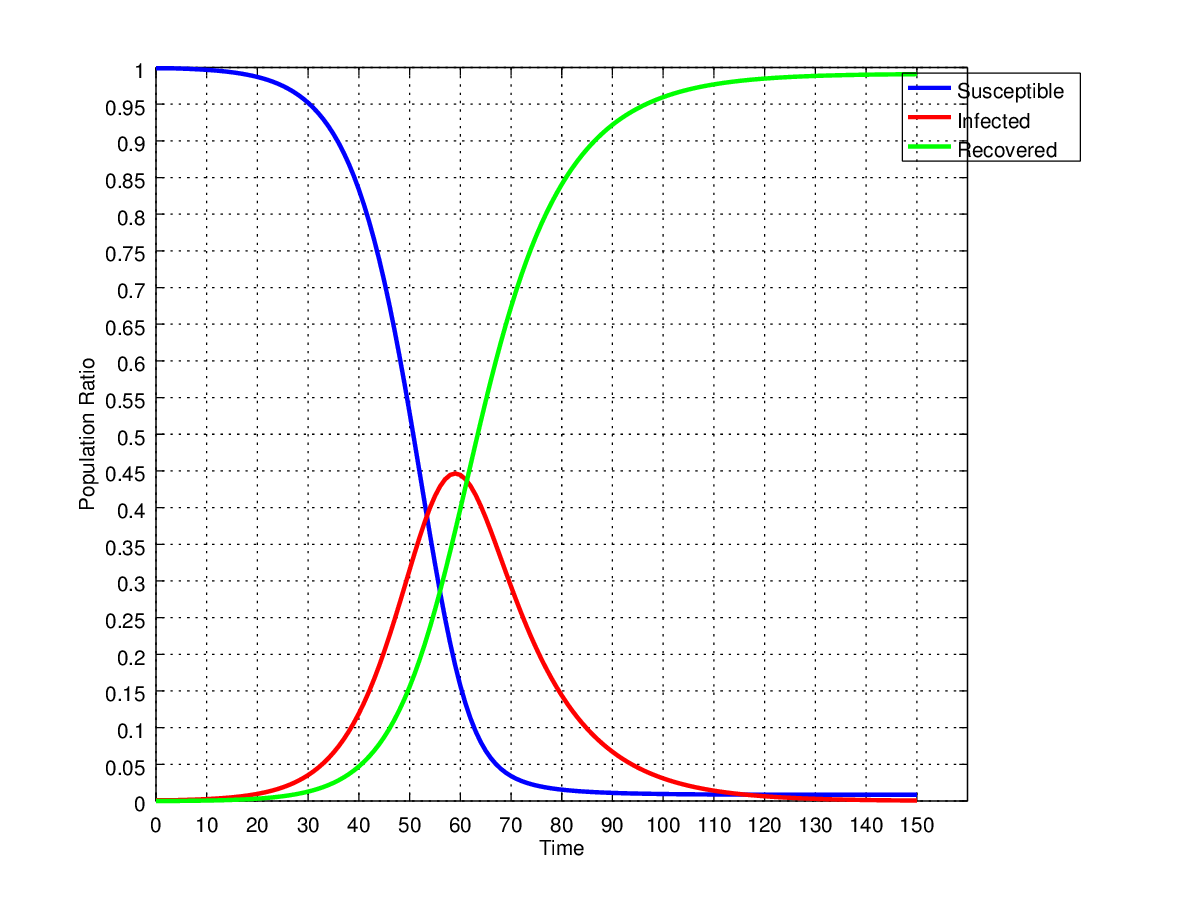
\includegraphics[width=.8\textwidth, angle=0]{./../shared/fig/frsd/SIR_SD_1000agents_150t_1dt.png}
			\caption{$\Delta t = 1.0$}
			\label{fig:sd_plot_10dt}
		\end{subfigure}
	
		& 
		
		\begin{subfigure}[b]{0.5\textwidth}
			\centering
			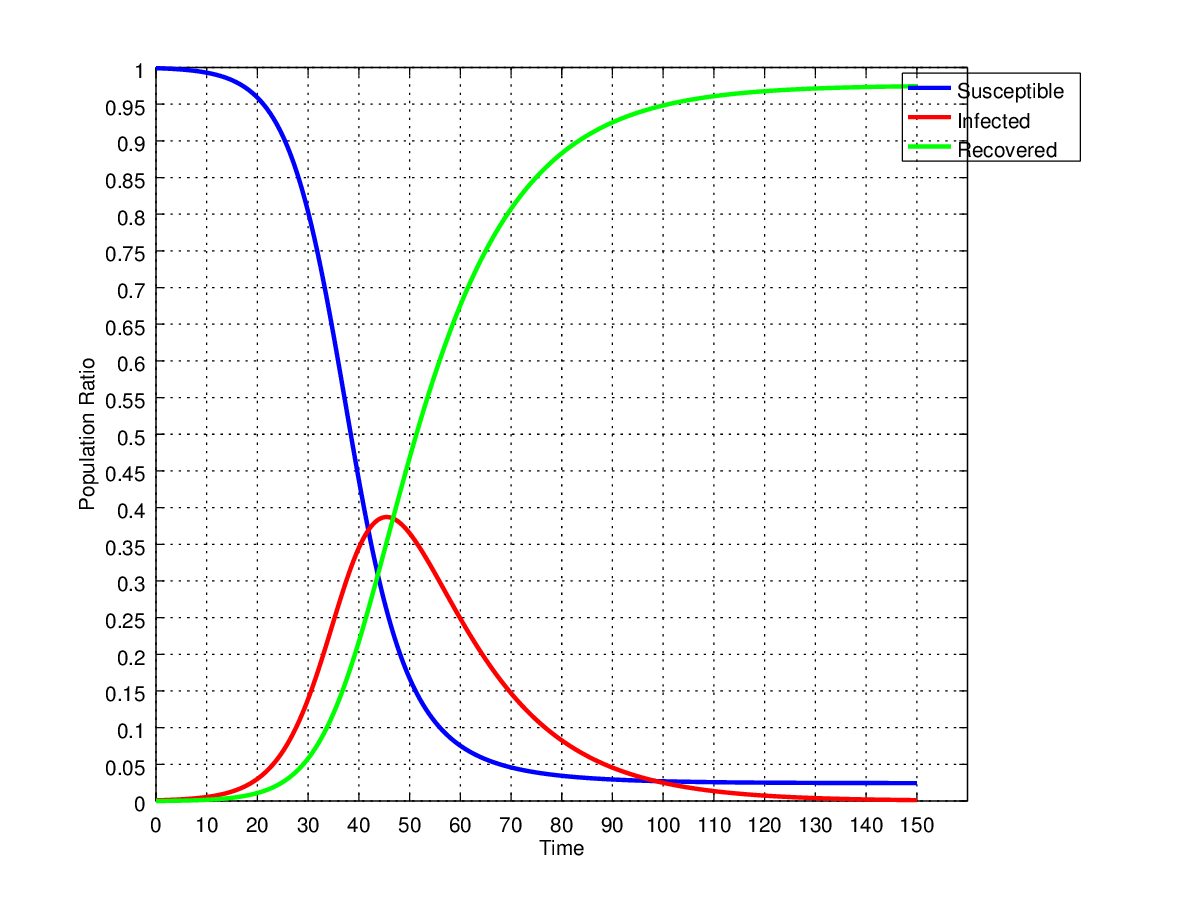
\includegraphics[width=.8\textwidth, angle=0]{./../shared/fig/frsd/SIR_SD_1000agents_150t_01dt.png}
			\caption{$\Delta t = 0.1$}
			\label{fig:sd_plot_0.1dt}
		\end{subfigure}
	\end{tabular}
	
	\caption{Simulating the SIR model with our SD emulation using different $\Delta t $. Note that although $\Delta t = 0.1$ might seem very close the system dynamic solution, there are still subtle differences to the initial Figure \ref{fig:sir_sd_dynamics} which uses $\Delta t = 0.01$.}
	\label{fig:sd_plots}
\end{center}
\end{figure*}

\subsection{Recursive ABS}
Due to the inherent recursive nature of functional programming we came up with the idea of \textit{recursive} ABS in which agents can recursively run the simulation within the simulation which would allow them to project their own actions into the future. So far it only exists as a proof-of-concept and we are currently only aware of a single model \cite{gilmer_recursive_2000} in the field of ABS which does recursive simulation. The implementation of recursive ABS is very natural due to the explicit data-flow and lack of side-effects which eases the task very much. Unfortunately we cannot go into detail of our approach as it is beyond the scope of the paper.


\subsection{Different Agent-Types}
[ ] can we implement different types of agents interacting with each other in the same simulation ? with different behaviour funcs, digferent state? yes, also not possible in NetLogo to my knowledge. but they must have the same messages, emvironment 

\subsection{Advantages}
	- no side-effects within agents leads to much safer code
	- edsl for time-semantics
	- declarative style: agent-implementation looks like a model-specification
	- reasoning and verification
	- sequential and parallel
	- powerful time-semantics
	- arrowized programming is optional and only required when utilizing yampas time-semantics. if the model does not rely on time-semantics, it can use monadic-programming by building on the existing monadic functions in the EDSL which allow to run in the State-Monad which simplifies things very much
	- when to use yampas arrowized programing: time-semantics, simple state-chart agents 
	- when not using yampas facilities: in all the other cases e.g. SugarScape is such a case as it proceeds in unit time-steps and all agents act in every time-step
	- can implement System Dynamics building on Yampas facilities with total ease	
	- get replications for free without having to worry about side-effects and can even run them in parallel without headaches
	- cant mess around with time because delta-time is hidden from you (intentional design-decision by Yampa). this would be only very difficult and cumbersome to achieve in an object-oriented approach. TODO: experiment with it in Java - how could we actually implement this? I think it is impossible: may only achieve this through complicated application of patterns and inheritance but then has the problem of how to update the dt and more important how to deal with functions like integral which accumulates a value through closures and continuations. We could do this in OO by having a general base-class e.g. ContinuousTime which provides functions like updateDt and integrate, but we could only accumulate a single integral value.
	- reproducibility statically guaranteed
	- cannot mess around with dt
	- code == specification
	- rule out serious class of bugs
	- different time-sampling leads to different results e.g. in wildfire \& SIR but not in Prisoners Dilemma. why? probabilistic time-sampling?
	- reasoning about equivalence between SD and ABS implementation in the same framework
	- recursive implementations
	
	- we can statically guarantee the reproducibility of the simulation because: no side effects possible within the agents which would result in differences between same runs (e.g. file access, networking, threading), also timedeltas are fixed and do not depend on rendering performance or userinput	
	
\subsection{Disadvantages}
	- performance is low
	- reasoning about performance is very difficult
	- very steep learning curve for non-functional programmers
	- learning a new EDSL
	- think ABMS different: when to use async messages, when to use sync conversations


[ ] important: increasing sampling freqzency and increasing number of steps so that the same number of simulation steps are executed should lead to same results. but it doesnt. why?
[ ] hypothesis: if time-semantics are involved then event ordering becomes relevant for emergent patterns. there are no tine semantics in heroes and cowards but in the prisoners dilemma
[ ] can we implement different types of agents interacting with each other in the same simulation ? with different behaviour funcs, digferent state? yes, also not possible in NetLogo to my knowledge. but they must have the same messages, emvironment 

[ ] Hypothesis: we can combine with FrABS agent-based simulation and system dynamics